\documentclass{beamer}
\usetheme{Warsaw}

\usepackage[utf8]{inputenc}
\usepackage{fancybox}
\usepackage{multimedia} 
\usepackage{subfig}
\usepackage{amsmath}
\usepackage{hyperref}
\usepackage[all]{xy}
\usepackage{algorithm}
%\usepackage{arevmath}     % For math symbols
\usepackage[noend]{algpseudocode}

\begin{document}


\title[Angewandte Mathematik] % (optional, only for long titles)
{Angewandte Mathematik
\\
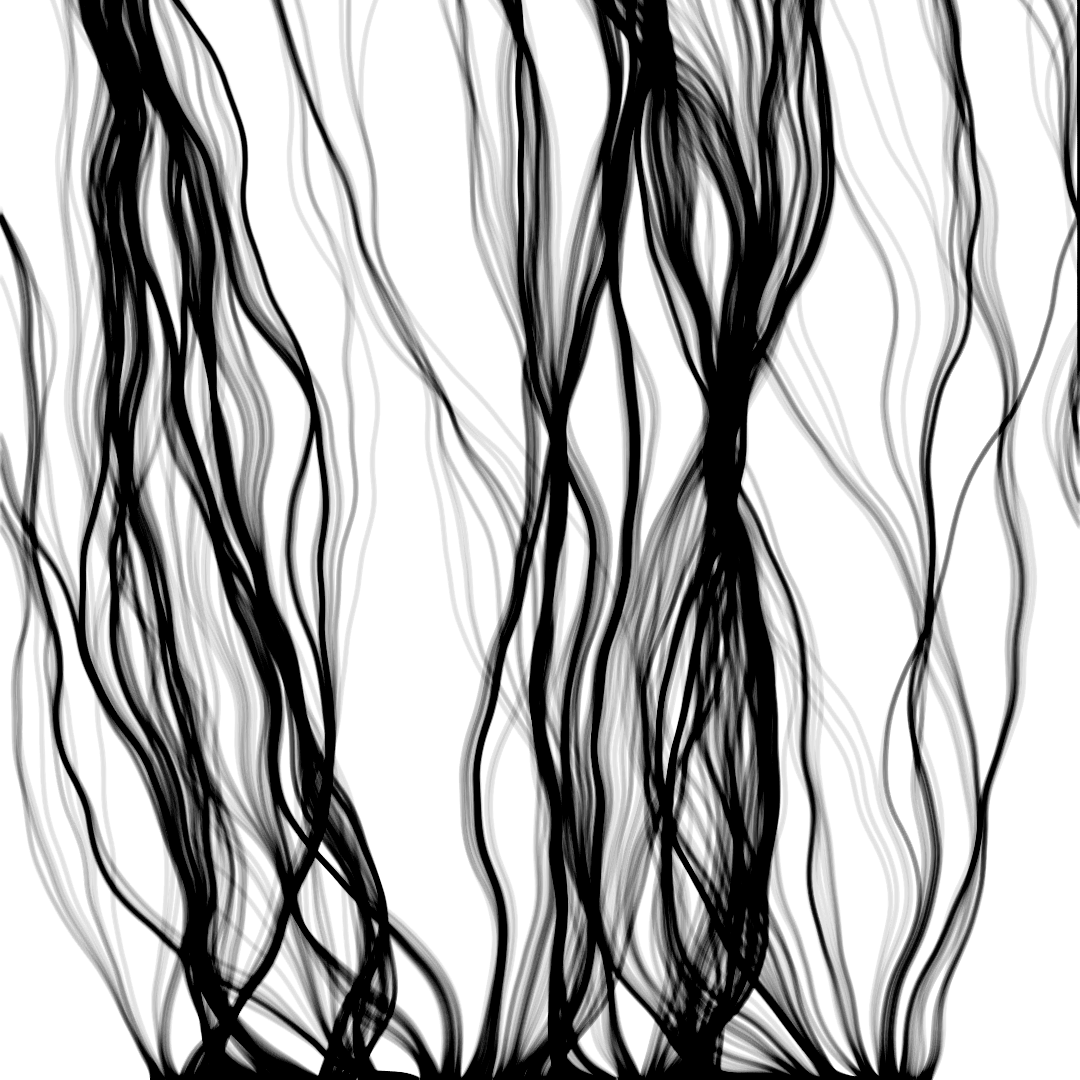
\includegraphics[scale=0.15]{images/cover}
}
\subtitle{}
\author[Dr. Johannes Riesterer] % (optional, for multiple authors)
{Dr.  rer. nat. Johannes Riesterer}

\date[KPT 2004] % (optional)
{}

\subject{Angewandte Mathematik}



\frame{\titlepage}



\begin{frame}
    \frametitle{Angewandte Mathematik}
\framesubtitle{Lebesgue Integral}
    \begin{block}{Indikatorfunktion}
Für eine Teilmenge $A \subset \mathbb{R}^n$ heißt
$$ 1_A (x): = \begin{cases} 1 \text{  falls }   x \in A  \\  0  \text{  sonst}  \end{cases}$$
Indikatorfunktion.
\end{block}

\begin{figure}[H]
      \centering
    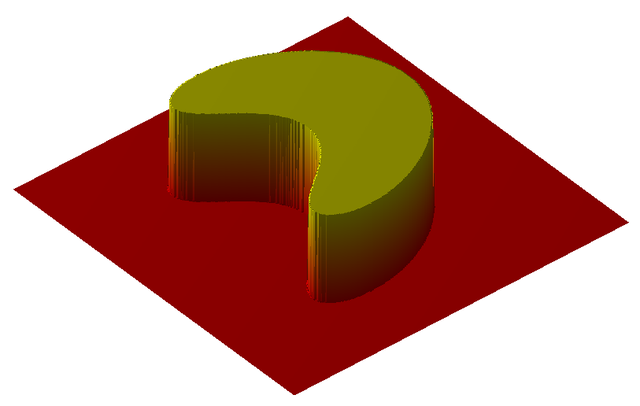
\includegraphics[width=0.6\textwidth]{images/640px-Indicator_function_illustration}
      \caption{Quelle: Wikipedia: https://commons.wikimedia.org/wiki/File:Indicator\_function\_illustration.png}

\end{figure}

 \end{frame}


\begin{frame}
    \frametitle{Angewandte Mathematik}
\framesubtitle{Lebesgue Integral}
    \begin{block}{Sinnvoller Integralbegriff}
Definiere Integral über Funktionen so, dass $\int 1_A d \mu = \mu(A)$
\end{block}

 \end{frame}

\begin{frame}
    \frametitle{Angewandte Mathematik}
\framesubtitle{Lebesgue Integral}
    \begin{block}{Indikatorfunktion}
Eine Funktion 
$$ \varphi(x) := \sum_{k=1}^m c_k 1_{I_k}$$ mit $c_k \in \mathbb{R}$ und $I_k \in \mathbb{I}(n)$ mit $I_l \cap I_h = \emptyset$ für $i \neq j$
heißt Treppenfunktion.
\end{block}


\begin{figure}[H]
      \centering
    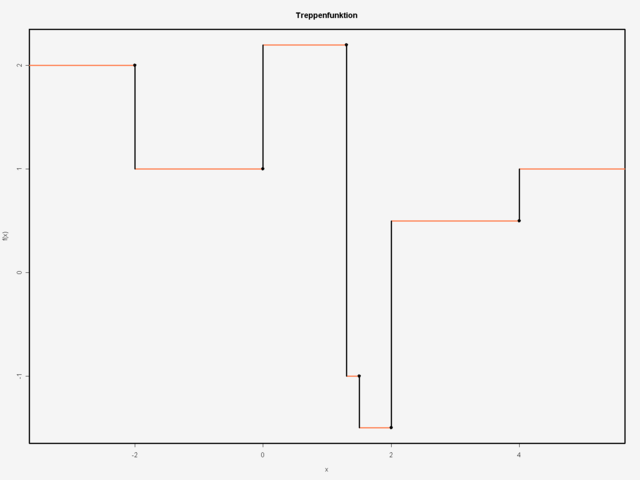
\includegraphics[width=0.4\textwidth]{images/640px-Stepfunction1}
      \caption{Quelle: Wikipedia: https://commons.wikimedia.org/wiki/File:Stepfunction1.png}

\end{figure}
 \end{frame}


\begin{frame}
    \frametitle{Angewandte Mathematik}
\framesubtitle{Lebesgue Integral}
    \begin{block}{Vektorraum der Indikatorfunktionen}

Seien $\varphi(x) =   \sum_{k=1}^m  c_k 1_{I_k}$ und $\psi(x) =  \sum_{j=1}^l  u_j 1_{I_j}$. Dann definiert
$(\varphi + \psi)(x) := \sum_{k=1}^m \sum_{j=1}^l   (c_k + u_j) 1_{I_{k,j}}$ mit $I_{k,j}:= I_k \cap I_j$ eine Treppenfunktion (nach entsprechender Umnummerierung zu einem einzigen Summenzeichen).
\end{block}

 \end{frame}


\begin{frame}
    \frametitle{Angewandte Mathematik}
\framesubtitle{Lebesgue Integral}
    \begin{block}{Integral von Treppenfunktionen}
Für eine Treppenfunktion $ \varphi(x) := \sum_{k=1}^m c_k 1_{I_k}$ definieren wir das Integral durch
$$\int_{\mathbb{R}^n} \varphi d\mu := \sum_{k =1}^m  c_k \mu(I_k) \; . $$
\end{block} 
\end{frame}


\begin{frame}
    \frametitle{Angewandte Mathematik}
\framesubtitle{Lebesgue Integral}
    \begin{block}{Eigenschaften des Integrals von Treppenfunktionen}
Seien $\varphi(x) =   \sum_{k=1}^m  c_k 1_{I_k}$ und $\psi(x) =  \sum_{j=1}^l  u_j 1_{I_j}$ zwei Treppenfunktionen.
Für das Integral von Treppenfunktion gilt:
\begin{itemize}
\item Ist $\varphi(x) = \psi(x)$ für alle $x$, dann ist $\int_{\mathbb{R}^n} \varphi d\mu = \int_{\mathbb{R}^n} \psi d\mu$ (Das integral hängt nicht von der Zerlegung der Treppenfunktion ab und  ist wohldefiniert)
\item $\int_{\mathbb{R}^n} \alpha \varphi  + \beta \psi d\mu = \alpha \int_{\mathbb{R}^n}  \varphi d\mu + \beta  \int_{\mathbb{R}^n}  \psi d\mu$
\item $ \biggl|  \int_{\mathbb{R}^n} \varphi d\mu  \biggr| \leq \int_{\mathbb{R}^n} | \varphi | d\mu$
\item Ist $\varphi(x) \leq \psi(x)$ für alle $x$, so ist $\int_{\mathbb{R}^n} \varphi d\mu \leq \int_{\mathbb{R}^n} \psi d\mu$ 
\end{itemize}
\end{block}

 \end{frame}


\begin{frame}
    \frametitle{Angewandte Mathematik}
\framesubtitle{Beweis}

Der Beweis wird über eine vollständige Induktion geführt. Der Induktionsanfang ist einfach zu zeigen. 
Wir nehmen an, die Aussage gilt für alle Dimensionen $k < n$.
Zerlege $\mathbb{R}^n = \mathbb{R}^p \times \mathbb{R}^{n-p}$. Jeder Quader $I \in \mathbb{I}(n)$ zerlegt sich damit ebenfalls in ein Produkt 
$I = I' \times I''$ mit $I'  \in \mathbb{I}(p)$ und  $I''  \in \mathbb{I}(n-p)$ und für $z = (x,y) \in  \mathbb{R}^p \times \mathbb{R}^{n-p}$ gilt $1_{I} (z) = 1_{I'}(x) \cdot 1_{I''}(y)$. Es sei nun $\varphi(z):=   \sum_{k=1}^m  c_k 1_{I_k}(z)$ eine Treppenfunktion auf $ \mathbb{R}^p \times \mathbb{R}^{n-p}$. Für jedes $y \in \mathbb{R}^{n-p}$ definiert  $\varphi_y(x)=   \sum_{k=1}^m  c_k 1_{I''_k}(y) \cdot 1_{I'_k}(x)$ eine Treppenfunktion auf $\mathbb{R}^{n-p}$. 
Nach Induktionsvoraussetzung hängt das Integral 
$$\int_{\mathbb{R}^p}  \varphi_y(x) d \mu' = \sum_{k=1}^m  c_k \mu'(I'_k)  \cdot 1_{I''_k}(y)  =: \phi(y)$$
nicht von der Zerlegung der Treppenfunktion ab.  \end{frame}

\begin{frame}
    \frametitle{Angewandte Mathematik}
\framesubtitle{Beweis}

$\phi(y)$ ist wiederum eine Treppenfunktion auf $\mathbb{R}^{n-p}$ und Nach Induktionsvoraussetzung hängt das Integral 
$$\int_{\mathbb{R}^{n-p}}  \phi(y) d \mu'' = \sum_{k=1}^m  c_k \mu'(I'_k)  \cdot \mu'' (I''_k)(y) $$
nicht von der Zerlegung der Treppenfunktion ab. Somit gilt
\begin{align*}
\int_{\mathbb{R}^{n-p}} \int_{\mathbb{R}^p}  \varphi_y(x) d \mu'  d \mu''  & =   \sum_{k=1}^m  c_k \mu'(I'_k)  \cdot \mu''(I''_k)(y) \\
& = \sum_{k=1}^m  c_k  \mu(I_k)  = \int_{\mathbb{R}^n} \varphi(z) d\mu\;.
\end{align*}
Die linke Seite hängt  damit nicht von der Zerlegung der Treppenfunktion ab und alle Behauptungen können so auf den Fall $n=1$ zurückgeführt werden.
 \end{frame}


\begin{frame}
    \frametitle{Angewandte Mathematik}
\framesubtitle{Lebesgue Integral}
    \begin{block}{Satz von Fubini für Treppenfunktionen}
Es gilt $$\int_{\mathbb{R}^n} \varphi(x,y) d \mu = \int_{\mathbb{R}^{n-p}} \biggl (\int_{\mathbb{R}^{p}}  \varphi(x,y) d \mu' \biggr ) d \mu''$$
\end{block}
    \begin{block}{Beweis}
Folgt direkt aus Beweis des letzten Satzes.
\end{block}
 \end{frame}


\begin{frame}
    \frametitle{Angewandte Mathematik}
\framesubtitle{Lebesgue Integral}
    \begin{block}{Hüllreihe}
Eine Hüllreihe zu einer Funktion $f :\mathbb{R}^n \to \mathbb{R}$ ist eine Reihe $\phi(x):= \sum_{k=1}^{\infty} c_k  1_{I_k} (x)$ mit den folgenden Eigenschaften:
\begin{itemize}
\item $c_k \in \mathbb{R}$ sind positive reelle Zahlen $c_k >0$.
\item $I_k \subset \mathbb{R}^n$ sind offene Quader.
\item Für alle $x \in \mathbb{R}^n$ gilt $|f(x) | \leq \phi(x)$.
\end{itemize}
\end{block}

 \begin{block}{Inhalt einer Hüllreihe}
Der Innhalt einer Hüllreihe $\phi(x):= \sum_{k=1}^{\infty} c_k  1_{I_k} (x)$ ist definiert durch 
$$I (\phi) := \sum_{k=1}^{\infty} c_k \;  \mu(I_k) \; .$$
\end{block}

 \end{frame}


\begin{frame}
    \frametitle{Angewandte Mathematik}
\framesubtitle{Lebesgue Integral}
    \begin{block}{ $L^1$-Halbnorm }
Die $L^1$-Halbnorm einer Funktion $f :\mathbb{R}^n \to \mathbb{R}$ is definiert durch das Infimum der Inhalte der Hüllreihen zu $f$
$$ || f ||_1 : = \inf  \biggl \{   I(\phi) \; | \; \phi  \text{ ist Hüllreihe zu  }  f \biggr \} \; .$$
\end{block}

 \end{frame}






\begin{frame}
    \frametitle{Angewandte Mathematik}
\framesubtitle{Lebesgue Integral}
    \begin{block}{Rechenregeln für Treppenfunktionen}
Für $f,g : \mathbb{R}^n \to \mathbb{R}$ und $c \in \mathbb{R}$ gilt:
 \begin{itemize}
\item $|| cf ||_1 \leq |c| || f ||_1$. 
\item $|| f +g ||_1 \leq  ||f ||_1 + ||g||_1$
\item Aus $|| f (x)||_1 \leq g(x)$ für alle $x$ folgt $|| f ||_1 \leq || g ||_1$.
\end{itemize}

\end{block}
 \end{frame}


\begin{frame}
    \frametitle{Angewandte Mathematik}
\framesubtitle{Beweis}
 \begin{itemize}
\item Für eine Hüllreihe $\varphi$ von $f$ ist $|c| \cdot \varphi$ eine Hüllreihe von $c \cdot f$. 
\item Da $|f +g | \leq | f | + | g |$ folgt Behauptung aus (iii) und der verallgemeinerten Dreiecksungleichung.
\item Hullreihen sind immer größer-gleich der Funktion und damit haben größere Funktionen größere Hüllreihen.
\end{itemize}
 \end{frame}



\begin{frame}
    \frametitle{Angewandte Mathematik}
\framesubtitle{Lebesgue Integral}
    \begin{block}{Verallgemeinerte Dreiecksungleichung}
Für nicht negative Funktionen $f_k  :\mathbb{R}^n \to \mathbb{R}_{\geq 0}$ gilt
$$ \biggl | \biggl | \sum_{k=1}^{\infty} f_k \biggr | \biggr |_1 \leq  \sum_{k=1}^{\infty} || f_k  ||_1 \; .$$
\end{block}

 \end{frame}



\begin{frame}
    \frametitle{Angewandte Mathematik}
\framesubtitle{Beweis}
$ 1 \cdot 1_I$ ist eine Hüllfunktion von $1_i$ und damit gilt $|| 1_I || \leq \mu(I)$. 
Sei $\phi(x) = \sum_k c_k 1_{I_k} $ eine Hüllreihe von $1_i$ und $\epsilon >0$. Da $\phi(x) \geq 1$ gibt es für jedes $x$ einen Index $N(x)$ mit 
$\sum_{k=1}^{N(x)} c_k 1_{I_k} \geq 1 - \epsilon$. Da die $I_k$ offen sind, gibt es für jedes $x$ eine Umgebung $U(x)$, so dass letztere Gleichung gilt. Da $\bar{I}$ kompakt ist (beschränkt und abgeschlossen), überdecken endlich viele $U(x_1), \cdots , U(x_n)$ den Quader $I$. Mit $N:= \max \{ N(x_1), \cdots , N(x_n)$ folgt $\sum_{k=1}^N c_k 1_{I_k} \geq (1-\epsilon) 1_I$. Aus den Rechenregeln für Treppenfunktionen (iii) folgt
$$ I (\phi) = \sum_k c_k \mu(I_k) \geq \sum_{k=1}^N c_k \mu (I_k) \geq (1 - \epsilon) \mu(I) \;.$$
Mit $\epsilon \to 0$ folgt $I (\phi) \geq \mu(i)$ und damit insgesamt die Behauptung.  
 \end{frame}


\begin{frame}
    \frametitle{Angewandte Mathematik}
\framesubtitle{Lebesgue Integral}
    \begin{block}{Norm und Integral}
Für jede Treppenfunktion $\varphi$ auf $\mathbb{R}^n$ gilt
$$ || \varphi ||_1 = \int | \varphi | d \mu  \; .$$
\end{block}

 \end{frame}




\begin{frame}
    \frametitle{Angewandte Mathematik}
\framesubtitle{Lebesgue Integral}
    \begin{block}{Integrierbare Funktionen}
Eine Funktion $f : \mathbb{R}^n \to \mathbb{R}$ heißt integrierbar, falls eine Folge von Treppenfunktionen  $\varphi_k$ existiert mit
$$ || f -  \varphi_k ||_1 \to 0 \text{ für } k \to \infty \;. $$
\end{block}

    \begin{block}{Integrierbare Funktionen}
\begin{itemize}
\item Die reelle Zahlenfolge $\int \varphi_k d\mu$ ist eine Cauchyfolge und damit konvergent. 
\item Der Grenzwert ist unabhängig von der Folge $\varphi_k$.
\end{itemize}
\end{block}


 \end{frame}






\begin{frame}
    \frametitle{Angewandte Mathematik}
\framesubtitle{Lebesgue Integral}
    \begin{block}{Vektorraum der Indikatorfunktionen}

\end{block}

 \end{frame}



\begin{frame}
    \frametitle{Angewandte Mathematik}
\framesubtitle{Beweis}

 \end{frame}



\end{document}

